\documentclass{article}
\usepackage[utf8]{inputenc}
\usepackage[left=3cm, right=3cm, top=2cm]{geometry}
\title{Documentation Edinburgh + Energy Analysis Tutorial}
\author{Silvin Willemsen}
\date{January 2019}

\usepackage{natbib}
\usepackage{graphicx}
\usepackage{appendix}
\usepackage{amsmath}
\usepackage{amsfonts}
\usepackage{amssymb}
\begin{document}

\maketitle

\section{Introduction}\label{sec:introduction}
The goal of my visit to the University of Edinburgh was to learn more about \textit{energy analysis}, a valuable technique to "debug" physical models. More specifically:

\begin{center}
    \textit{The purpose of the visit to the University of Edinburgh is to fully understand the concept of energy analysis and be able to apply it to arbitrary (connected) physical models. The goal will have been fulfilled if I can carry out an energy analysis on a string and a plate connected by a non-linear spring.}
\end{center}

This document shows what I learned during my two weeks at the University of Edinburgh. It will contain a tutorial on performing energy analysis for (my) future reference. 

Stefan Bilbao's \textit{Numerical Sound Synthesis} \cite{Bilbao2009} will be used as the main reference for this document. Whenever referred to an Equation, Section or Chapter, it can be assumed that this can be found in Bilbao's book. References to equations or sections in this document can be identified by only having one number (e.g. Eq. \eqref{eq:1DWave} instead of Eq. (6.1)) unless specified otherwise.

% \begin{figure}[h!]
% \centering
% 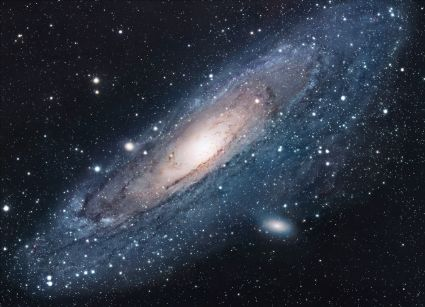
\includegraphics[scale=1.7]{universe}
% \caption{The Universe}
% \label{fig:universe}
% \end{figure}

\section{Notation}\label{sec:notation} 
The notation used in this document will be the one used in \cite{Bilbao2009}. 

\subsection{Difference Operators} 
% This section is divided into two: operators in 1D and operators in 2D.
Timeshifts (Sec 2.2)
\begin{equation}
    e_{t+}u_l^n = u_l^{n+1}, \quad e_{t-}u_l^n = u_l^{n-1}
\end{equation}
\subsubsection{Operators in 1D}\label{subsec:1Doperators}
Applied to state variable $u = u(x,t)$, the following abbreviated notation for partial differential operators in continuous time will be used (Sec. 5.1):
\begin{equation}\label{eq:PDA}
    \frac{\partial u}{\partial t} = u_{t}, \quad \frac{\partial^2 u}{\partial t^2} = u_{tt}, \quad
    \frac{\partial u}{\partial x} = u_{x}, \quad \frac{\partial^2 u}{\partial x^2} = u_{xx}, \quad
    \frac{\partial^4 u}{\partial x^4} = u_{xxxx}, \quad
    \text{etc}.
\end{equation}
In discrete time, the state variable $u$ will be 'subdivided' into points in time and space. Here this will happen at times $t = nk$, where $n \in \mathbb{N}$ and $k = 1 / f_\text{s}$ is the time-step with sample-rate $f_\text{s}$ and locations $x = lh$, where $l \in [0,N]$ with $N$ being the total number of points and $h$ is the grid-spacing of the model we need to approximate the derivatives. The discretised variable $u_l^n$ is $u(x,t)$ at the $n$th time step and the $l$th point on the string.

It is useful to use an operator notation for this (see Sec 2.2). For example, $u_t$ can be approximated in different ways (Eq. 2.3a-c):
\begin{subequations}\label{eq:firstOrderTime}
\begin{align}
    u_t &\approx \delta_{t+}u_l^n = \frac{1}{k} (u_l^{n+1} - u_l^n),\\
    u_t &\approx \delta_{t-}u_l^n = \frac{1}{k} (u_l^n - u_l^{n-1}),\\
    u_t &\approx \delta_{t\cdot}u_l^n = \frac{1}{2k} (u_l^{n+1} - u_l^{n-1}).
\end{align}
\end{subequations}
These are commonly referred to as the forward, backward and centered difference approximations (Sec 2.2). The second time-derivative may be approximated using a combination of these operators (Eq. 2.4):
\begin{equation}\label{eq:secondOrderTime}
u_{tt} \approx \delta_{tt}u_l^n = \delta_{t+}\delta_{t-}u_l^n = \frac{1}{k^2} (u_l^{n+1}-2u_l^n+u_l^{n-1}).
\end{equation}
Next to this, averaging operators are essential in energy analysis and discretisation of connections which will be shown in Section \ref{sec:energy}. These can be defined as:
\begin{align}
    \mu_{t+}u_l^n &= \frac{1}{2} (u_l^{n+1} + u_l^n),\\
    \mu_{t-}u_l^n &= \frac{1}{2} (u_l^n + u_l^{n-1}),\\
   \mu_{t\cdot}u_l^n &= \frac{1}{2} (u_l^{n+1} + u_l^{n-1}).
\end{align}
Note that rather than subtracting two time instances of $u$ they are added. Additionally, instead of dividing by time-step $k$, they are divided by 2, even the centered averaging operator. Also these operators can be combined:

\begin{equation}
    \mu_{tt} u_l^n = \mu_{t+}\mu_{t-}u_l^n = \frac{1}{4}(u_l^{n+1}+2u_l^n+u_l^{n-1})
\end{equation}
All of the above can be done for spatial partial derivatives (Sec 5.2.2). For the first order 
\begin{subequations}\label{eq:firstOrderSpace}
\begin{alignat}{2}
    u_x &\approx \delta_{x+}u_l^n &&= \frac{1}{h} (u_{l+1}^n - u_l^n),\\
    u_x &\approx \delta_{x-}u_l^n &&= \frac{1}{h} (u_l^n - u_{l-1}^n),\\
    u_x &\approx \delta_{x\cdot}u_l^n &&= \frac{1}{2h} (u_{l+1}^n - u_{l-1}^n),
\end{alignat}
\end{subequations}
and second order 
\begin{equation}\label{eq:secondOrderSpace}
    u_{xx} \approx \delta_{xx}u_l^n = \delta_{x+}\delta_{x-}u_l^n = \frac{1}{h^2} (u_{l+1}^n - 2u_l^n + u_{l-1}^n).
\end{equation}

\subsubsection{Operators in 2D}\label{subsec:2Doperators}
In 2D, the collection of partial differential abbreviations shown in \eqref{eq:PDA} can be extended with the following (Sec. 10.1.3)

\begin{equation}
    \frac{\partial u}{\partial y} = u_{y}, \quad \frac{\partial^2 u}{\partial y^2} = u_{yy}, \quad
    \frac{\partial^2 u}{\partial x\partial y} = u_{xy}, \quad
    \frac{\partial^4 u}{\partial x^2\partial y^2} = u_{xxyy}, \quad
    \frac{\partial^4 u}{\partial y^4} = u_{yyyy},
\end{equation}
A commonly used operator to denote a second order spatial derivative in both $x$ and $y$ direction is the Laplacian operator. When applied to a state $u=u(x,y,t)$ this results in (Eq. 10.2)
\begin{equation}
    \Delta u = u_{xx} + u_{yy}.
\end{equation}
When applied twice, this is called the biharmonic or bi-Laplacian operator and results in (Eq. 10.3) \begin{equation}
    \Delta\Delta u = u_{xxxx} + 2u_{xxyy} + u_{yyyy}.
\end{equation}
In discrete time we can approximate the above operators (Sec. 10.2, Eq. 10.9:
\begin{equation}
    \Delta u \approx \delta_{\Delta\boxplus} \triangleq \delta_{xx}u + \delta_{yy}
\end{equation}
and 
\begin{equation}
    \Delta\Delta u \approx \delta_{\Delta\boxplus}\delta_{\Delta\boxplus} \triangleq \delta_{xxxx}u + 2\delta_{xxyy} + \delta_{yyyy}
\end{equation}

\subsection{Inner Products and Norms}
A spatial inner product of functions $f$ and $g$ over a domain $\mathcal{D}$ is equivalent to taking the integral of the product of these functions. In continuous time is written as (Eq. 5.6)
\begin{equation}
    \langle f,g\rangle_\mathcal{D} = \int_\mathcal{D}fgdx, 
\quad \text{and} \quad 
    \langle f,f \rangle_\mathcal{D} = \left\lVert f \right\rVert^2_\mathcal{D}.
\end{equation}
In discrete time this becomes (Eq. 5.20)
\begin{equation}\label{eq:innerProduct}
     \langle f^n,g^n\rangle_\mathcal{D} = \sum_{l\in\mathcal{D}}h f^n_l g^n_l \quad \text{and} \quad \left\lVert f^n \right\rVert^2_\mathcal{D} = \sum_{l\in\mathcal{D}}h(f^n_l)^2.
\end{equation}
Note the multiplication with the grid spacing $h$ in the sum.
\subsection{Energy}
For the total energy in continuous time we use $\mathfrak{H}$ which is mostly an addition of the kinetic energy denoted by $\mathfrak{T}$ and the potential energy denoted by $\mathfrak{D}$. In discrete time these will be $\mathfrak{h}$, $\mathfrak{t}$ and $\mathfrak{v}$ %why not d though??
respectively.
\section{Physical Models}
I learned that there are two ways of approaching a partial differential equation (PDE) of a physical model:
\begin{itemize} 
    \item Dimensional form,
    \item Non-Dimensional or (Spatially) Scaled form.
\end{itemize}
To illustrate this we start with the 1D wave equation (Eq. (6.1)) where the dimensional form is defined as
\begin{equation}\label{eq:1DWave}
    \rho A u_{tt} = T u_{xx}, 
\end{equation}
with material density $\rho$ [kg/m$^3$], cross-sectional area $A$ [m$^2$] and string tension $T$ [N].
The scaled form of is defined ase
\begin{equation}\label{eq:1DWaveScaled}
    u_{tt} = \gamma^2 u_{x'x'},
\end{equation}
where $\gamma = c/L$ is the scaled wave speed [s$^{-1}$] with (non-scaled) wave speed $c = \sqrt{T/\rho A}$ [m/s] and string-length $L$ [m].

In the first case, $x$ is defined over a physical domain $x\in[0,L]$. In the scaled case, $x' = x/L$ is a unit-less variable defined over $x\in[0,1]$. An advantage of scaling is that it greatly simplifies the the physical system one works with \cite{Bilbao2009}. However, in my application, when working with two  elements of different types, it is better to take a step back to the slightly less simple, but more physically accurate world. In the rest of this documents I will thus use a dimensional form for the equations.

\subsection{Ideal Stiff String}
The PDE for a stiff string is a combination of the 1D wave equation (Eq. \eqref{eq:1DWave}) and the ideal bar model (Eq. 7.1):
\begin{equation}\label{eq:stiffStringPDE}
    \rho A u_{tt} = T u_{xx} - EI u_{xxxx},
\end{equation}
with Young's Modulus $E$ [kg $\cdot$m$^{-1} \cdot$s$^{-2}$] and moment of inertia $I$ [kg$\cdot$m$^2$]. The latter can be calculated using $I = \pi r^4/4$ for a cylindrical object [Check with Stefan].

Using the difference operators presented in Subsection \ref{subsec:1Doperators} (of this document) we can discretise Eq. \eqref{eq:stiffStringPDE} into the following finite-difference scheme (FDS):
\begin{equation}\label{eq:stiffStringFDS}
    \rho A \delta_{tt}u_l^n = T \delta_{xx} u_l^n - EI \delta_{xxxx} u_l^n.
\end{equation}
For simplicity we will divide both sides by $\rho A$ and introduce stiffness factor $\kappa = \sqrt{EI/\rho A}$:
\begin{equation}\label{eq:stiffStringFDSVars}
   \delta_{tt}u_l^n = c^2 \delta_{xx} u_l^n - \kappa^2 \delta_{xxxx} u_l^n.
\end{equation}
Expanding the operators yields
\begin{equation}
    \frac{1}{k^2}(u_l^{n+1}-2u_l^n+u_l^{n-1}) = \frac{c^2}{h^2}(u_{l+1}^n-2u_l^n+u_{l-1}^n)- \\
 \frac{\kappa^2}{h^4}(u_{l+2}^n-4u_{l+1}^n+6u_l^n-4u_{l-1}^n+u_{l-2}^n)
\end{equation}
We can then solve for $u_l^{n+1}$ by multiplying both sides by $k^2$ and subtracting the terms of $u$ at the current and previous time step from both sides, resulting in the following update equation:
\begin{equation}
    u_l^{n+1} = 2u_l^n-u_l^{n-1}+\frac{c^2k^2}{h^2}(u_{l+1}^n-2u_l^n+u_{l-1}^n)-\frac{\kappa^2k^2}{h^4}(u_{l+2}^n-4u_{l+1}^n+6u_l^n-4u_{l-1}^n+u_{l-2}^n).
\end{equation}

\subsection{Plate}
The PDE for a thin plate is defined as (Eq. 12.1)
\begin{equation}\label{eq:platePDE}
    \rho H u_{tt} = -D\Delta\Delta u,
\end{equation}
where $D = EH^3/12(1-\nu^2)$ with plate thickness $H$ [m] and unit-less Poisson's ratio $\nu$. As with the stiff string, we can use the operators presented in Subsection \ref{subsec:2Doperators} (of this document) to discretise Eq. \eqref{eq:platePDE} into the following FDS: 
\begin{equation}\label{eq:plateFDS}
    \rho H \delta_{tt}u = -D\delta_{\Delta\boxplus}\delta_{\Delta\boxplus} u,
\end{equation}
and when introducing stiffness factor $\kappa =\sqrt{D/\rho H}$, \eqref{eq:plateFDS} becomes
\begin{equation}\label{eq:plateFDS}
    \delta_{tt}u = -\kappa^2\delta_{\Delta\boxplus}\delta_{\Delta\boxplus} u,
\end{equation}
Again, expanding the operators yields

\frac{1}{k^2}(u_l^{n+1}-2u_l^n+u_l^{n-1}) = -\frac{\kappa^2}\delta_{\Delta\boxplus}\frac{1}{h^4}


\section{Energy Analysis: A Tutorial}\label{sec:energy}
As mentioned in Section \ref{sec:introduction}, energy analysis is the only way to 'debug' physical models. In this section I will give an overview on how to do an energy analysis using the stiff string as a case study. 

\subsubsection*{Step 1: Calculate the rate of change of the total energy $\mathfrak{H}$} %(taking the inner product with a single time derivative of $u$
The rate of change of the total energy (or Hamiltonian (Sec. 3.1.2)) $\mathfrak{H}$ of a system over domain $\mathcal{D}$ can be obtained by calculating the inner product of a system with $u_t$ \cite{Desv2017}
\begin{equation}\label{eq:generalEnergy}
    \frac{d \mathfrak{H}}{dt} = \langle u_t, \text{PDE} \rangle_\mathcal{D} \quad \text{with} \quad \mathfrak{H} = \mathfrak{T} + \mathfrak{D},
\end{equation}
% The first step to obtaining the energy of a system is to the whole system needs to be multiplied with the single time derivative of $u$, i.e. the velocity of the state $u$.
where $\mathfrak{H}$ is the addition of its kinetic energy $\mathfrak{T}$ and its potential energy $\mathfrak{D}$ and PDE is a partial differential equation such as Eq. \eqref{eq:stiffStringPDE}. Furthermore, domain $\mathcal{D} \in [0,L]$. In a lossless system like Eq. \eqref{eq:stiffStringPDE} the energy will be constant. In other words the rate of change over time will be zero:
\begin{equation}\label{eq:energyZero}
    \frac{d \mathfrak{H}}{dt} = 0,
\end{equation}
In the case of the stiff string in continuous time (or choosing Eq. \eqref{eq:stiffStringPDE} for PDE) Eq. \eqref{eq:generalEnergy} yields
\begin{equation}\label{eq:stiffStringInnerProduct}
     \rho A \langle u_t, u_{tt}\rangle_\mathcal{D} = T \langle u_t, u_{xx}\rangle_\mathcal{D} - EI \langle u_t, u_{xxxx} \rangle_\mathcal{D}.
\end{equation}
In discrete time, Eq. \eqref{eq:generalEnergy} looks like %stefan said that you can not just assume this "\delta_{t+}\mathfrak{h} is what you HOPE to find by doing this
\begin{equation}\label{eq:generalEnergyDiscretised}
    \delta_{t+}\mathfrak{h} = \langle \delta_{t\cdot}u, \text{FDS}\rangle_\mathcal{D} \quad \text{with} \quad \mathfrak{h} = \mathfrak{t} + \mathfrak{v},
\end{equation}
where $\mathfrak{h}$, $\mathfrak{t}$ and $\mathfrak{v}$ are approximated (discretised) versions of $\mathfrak{H}$, $\mathfrak{T}$ and $\mathfrak{D}$ and FDS is a finite-difference scheme such as Eq. \eqref{eq:stiffStringFDS}. Note that we use $\delta_{t+}$ because (ask Stefan).
So in the case of a stiff string in discrete time (or choosing Eq. \eqref{eq:stiffStringFDS} for FDS) Eq. \eqref{eq:generalEnergyDiscretised} gives
\begin{equation}
     \rho A \langle \delta_{t\cdot}u, \delta_{tt} u\rangle_\mathcal{D} = T \langle \delta_{t\cdot}u, \delta_{xx}u\rangle_\mathcal{D} - EI \langle \delta_{t\cdot}u, \delta_{xxxx}u \rangle_\mathcal{D}.
\end{equation}
Note that for the approximation of $u_t$ the centered difference operator $\delta_{t\cdot}$ has been used. This is because it is the most accurate approximation of the single time derivative \cite{Bilbao2009}. Using integration by parts (Eq. 5.10 or Eq. 6.14 for its use in practice) and moving all terms to the left hand side gives us the rate of change of the total energy of the system:

\begin{equation}\label{eq:stiffStringEnergy}
     \delta_{t+}\mathfrak{h} = \rho A \langle \delta_{t\cdot}u, \delta_{tt} u\rangle_\mathcal{D} + T \langle \delta_{t\cdot}\delta_{x+}u, \delta_{x+}u\rangle_\mathcal{D} + EI \langle \delta_{t\cdot}\delta_{xx}u, \delta_{xx}u \rangle_\mathcal{D} = 0.
\end{equation}
In a certain sense, when moving a single spatial derivative from one term in the inner product to the other, the sign of that term inverts.

\subsubsection*{Step 2: Obtaining the total energy $\mathfrak{H}$ (Factoring out $\delta_{t+}$)}
% "In energetic analysis, whenever possible, it is useful to rewrite terms such as these as time derivatives of a single quantity" \cite{Bilbao2009}
Now that we obtained the rate of change of the total energy of our PDE, in order to get the actual energy it is necessary to factor out a single derivative with respect to time.
 In the case of the stiff string (or any other system), the goal is to rewrite Eq. \eqref{eq:stiffStringEnergy} into the form of
\begin{equation}\label{eq:forwardTimeForm}
    \delta_{t+}(\text{X}) = 0,
\end{equation}
where $\text{X}=\mathfrak{t} + \mathfrak{v}$.
As the first term can be expanded to
\begin{equation}
    \rho A\sum_\mathcal{D}h(\delta_{t\cdot}u)(\delta_{tt}u).
\end{equation}
When factoring out $\delta_{t+}$ we get (Eq. 2.22a)
\begin{equation}
\delta_{t+}\Bigg(\frac{\rho A}{2}\sum_\mathcal{D}h(\delta_{t-}u)^2\Bigg) = \delta_{t+}\Bigg(\frac{\rho A}{2} \left\lVert\delta_{t-}u\right\rVert_\mathcal{D}^2\Bigg).
\end{equation}
The second term can be expanded (using Eq. \eqref{eq:innerProduct}) to get
\begin{equation}
    T \sum_{\mathcal{D}}h (\delta_{t\cdot}\delta_{x+}u)(\delta_{x+}u).
\end{equation}
Again, factoring out $\delta_{t+}$ (Sec. 2.4.1)
\begin{equation}
    \delta_{t+}\Bigg(\frac{T}{2}\sum_\mathcal{D}h (\delta_{x+}u)( e_{t-}\delta_{x+}u)\Bigg) = \delta_{t+}\Bigg(\frac{T}{2}\langle\delta_{x+}u, e_{t-}\delta_{x+}u\rangle_\mathcal{D}\Bigg),
\end{equation}
where $e_{t-}$ denotes a backwards time shift (see Section \ref{sec:notation})
We can do the same with the last term. Expanding gives
\begin{equation}
    EI \sum_{\mathcal{D}}h(\delta_{t\cdot}\delta_{xx}u)(\delta_{xx}u),
\end{equation}
and factoring out $\delta_{t+}$ yields (Eq. 2.22b)
\begin{equation}
    \delta_{t+}\Bigg(\frac{EI}{2}\sum_\mathcal{D}h(\delta_{xx}u)(e_{t-}\delta_{xx}u)\Bigg) = \delta_{t+}\Bigg(\frac{EI}{2}\langle\delta_{xx}u,e_{t-}\delta_{xx}u\rangle_\mathcal{D}\Bigg).
\end{equation}
Now we can finally write Eq. \eqref{eq:stiffStringEnergy} in the form presented in Eq. \eqref{eq:forwardTimeForm}:
\begin{equation}
    \delta_{t+}\mathfrak{h} = \delta_{t+}\Bigg(\frac{\rho A}{2}\left\lVert\delta_{t-}u\right\rVert_\mathcal{D}^2 + \frac{T}{2}\langle\delta_{x+}u, e_{t-}\delta_{x+}u\rangle_\mathcal{D} +\frac{EI}{2}\langle\delta_{xx}u,e_{t-}\delta_{xx}u\rangle_\mathcal{D}\Bigg) = 0.
\end{equation}
Integrating both sides with respect to time (removing/dividing by? the $\delta_{t+}$ operator on both sides) yields the total energy $\mathfrak{h}$:
\begin{equation}\label{eq:totEnergyString}
    \mathfrak{h} = \frac{\rho A}{2}\left\lVert\delta_{t-}u\right\rVert_\mathcal{D}^2 + \frac{T}{2}\langle\delta_{x+}u, e_{t-}\delta_{x+}u\rangle_\mathcal{D} +\frac{EI}{2}\langle\delta_{xx}u,e_{t-}\delta_{xx}u\rangle_\mathcal{D},
\end{equation}
which is not necessarily 0! 

\subsubsection*{Step 3: Checking units}
In order to check whether the terms in the equation for total energy, in this case Eq. \eqref{eq:totEnergyString}, are correct, it is important to check their units. Energy is measured in Joules [kg$\cdot$m$^2\cdot$s$^{-2}$]. A first order temporal difference operator (Eqs. (\ref{eq:firstOrderTime}a-c)) will `add' one [s$^{-1}$] (because of the $1/k$) and a first order spatial difference operator (Eqs. (\ref{eq:firstOrderSpace}a-c)) will `add' one [m$^{-1}$] ($1/h$) unit. All states $u$ will `add' one [m] to the equation. Along these lines, a second order time or difference operator (Eqs. \eqref{eq:secondOrderTime} and \eqref{eq:secondOrderSpace}) will `add' a [s$^{-2}$] or [m$^{-2}$] respectively. It is important to note that the time shift operator ($e_{t-}$) does not influence the units. For units on several variables, see Appendix \ref{app:A}. For the terms above, we have:
\begin{subequations}
\begin{align}
\frac{\rho A}{2}\sum_\mathcal{D}h(\delta_{t-}u)^2 \quad
&\overset{\text{in units}}{\xrightarrow{\hspace*{1cm}}}    \quad\text{kg}\cdot\text{m}^{-3}\cdot\text{m}^2\cdot\text{m}\cdot(\text{s}^{-1}\cdot\text{m})^2 = \text{kg}\cdot\text{m}^2\cdot\text{s}^{-2}\\
\frac{T}{2}\sum_\mathcal{D}h (\delta_{x+}u)( e_{t-}\delta_{x+}u) \quad
&\overset{\text{in units}}{\xrightarrow{\hspace*{1cm}}}    \quad\text{kg}\cdot\text{m}\cdot\text{s}^{-2}\cdot\text{m}\cdot(\text{m}^{-1}\cdot\text{m})\cdot(\text{m}^{-1}\cdot\text{m}) = \text{kg}\cdot\text{m}^2\cdot\text{s}^{-2}\\
\frac{EI}{2}\sum_\mathcal{D}h (\delta_{xx}u)( e_{t-}\delta_{xx}u) \quad
&\overset{\text{in units}}{\xrightarrow{\hspace*{1cm}}}    \quad\text{kg}\cdot\text{m}^{-1}\cdot\text{s}^{-2}\cdot\text{m}^4\cdot\text{m}\cdot(\text{m}^{-2}\cdot\text{m})\cdot(\text{m}^{-2}\cdot\text{m}) = \text{kg}\cdot\text{m}^2\cdot\text{s}^{-2}
\end{align}
\end{subequations}

\subsubsection*{Step 4: Identifying kinetic and potential energies}
We can now identify what terms contribute to the the kinetic energy $\mathfrak{t}$ and potential energy $\mathfrak{v}$. The kinetic energy must be in the form of mass $\times$ velocity squared. The rest contributes to the potential energy. %by seeing whether they are spatially dependent. Not spatially dependent terms contribute to kinetic energy whereas spatially dependent terms contribute to potential energy. (CHECK IF THIS IS CORRECT) 
In the case of Eq. \eqref{eq:totEnergyString} this gives
\begin{equation}
    \mathfrak{t} = \frac{\rho A}{2}\sum_\mathcal{D}h(\delta_{t-}u)^2 \quad \text{and} \quad \mathfrak{v} = \frac{T}{2}\sum_\mathcal{D}h (\delta_{x+}u)( e_{t-}\delta_{x+}u) +\frac{EI}{2}\sum_\mathcal{D}h(\delta_{xx}u)(e_{t-}\delta_{xx}u).
\end{equation}

\subsubsection*{Step 5: Implementation}
Now that the total energy of the system has correctly been obtained, the next step is to put it to practice to check the model correctness. We can expand kinetic energy $\mathfrak{t}$ to
\begin{equation}
    \mathfrak{t} = \frac{\rho A}{2}\sum_{l=0}^Nh\bigg(\frac{1}{k}(u_l^n - u_l^{n-1})\bigg)^2.
\end{equation}
As calculating the potential energy requires grid-points left and right of $l$, we can not calculate the sum over all grid points. In other words, in order to calculate $\mathfrak{v}$ at $l = \{0, N\}$ (where $N$ is the number of grid points on the string) we need points $l = -1 \text{ and } l = N + 1$ which are out of bounds. Instead, we sum over a slightly smaller domain of $\mathcal{D} = [1, L - h]$ to keep the calculations within the bounds:
\begin{equation}
\begin{aligned}
   \mathfrak{v} = \frac{T}{2}\sum_{l = 1}^{N-1} h\frac{1}{h^2}(u_{l+1}^n - u_l^n)(u_{l+1}^{n-1} - u_l^{n-1})
   + \frac{EI}{2}\sum_{l = 1}^{N-1}h\frac{1}{h^4}(u_{l+1}^n-2u_l^n+u_{l-1}^n)(u_{l+1}^{n-1}-2u_l^{n-1}+u_{l-1}^{n-1})
\end{aligned}
\end{equation}
This is possible as the boundary conditions of the string have been chosen to be clamped, meaning the points at $u_l^n = 0$ at $l = \{0, 1, N-1, N\}$ for all $n$. Even though the displacement at points $l = \{1, N-1\}$ will always be zero, the energy is not necessarily zero. When calculating the energy for the aforementioned points, the points $l = \{2, N-2\}$ are included which are not necessarily $0$.

\section{Case study: Energy analysis of a string and plate connected by a non-linear spring}


\appendix
\section{List of symbols} \label{app:A}
{\renewcommand{\arraystretch}{1.1}
\begin{tabular}{ p{3cm} p{7cm} p{4cm}  }
 Symbol & Description & Unit\\
 \hline\\
 $A$ & Cross-sectional area & m$^2$\\
 $c$ & Wave speed & m$\cdot$s$^{-1}$\\
 $E$ & Young's Modulus & kg$\cdot$m$^{-1}\cdot$s$^{-2}$\\
 $f_\text{s}$ & Sample rate & s$^{-1}$\\
 $h$ & Grid-spacing & m \\ 
 $I$ & Area moment of inertia \cite{Desv2017} & m$^4$\\
 $L$ & String length & m\\
 $k$ & Time-step ($1/f_\text{s}$) & s\\
 $N$ & Number of points string & -\\
 $T$ & String tension & N (kg$\cdot$m$\cdot$s$^{-2}$) \\
 $u$ & State variable ($u(x,t)\text{ or }u(x,y,t)$) & m (displacement)\\ 
 $\kappa$ & Stiffness factor & m$^4\cdot$s$^{-2}$\\
 $\rho$ & Material density & kg$\cdot$m$^{-3}$\\
 $\gamma$ & Scaled wave speed & s$^{-1}$\\
\end{tabular}
}
\section{Code}

\bibliographystyle{plain}
\bibliography{references}
\end{document}


%Questions:
%Is the domain correct? 